\documentclass[11pt]{article}
\usepackage[margin=0.9in]{geometry}
\usepackage{amsmath,amssymb,mathtools}
\usepackage{booktabs,array,enumitem,microtype,xcolor,hyperref,fancyhdr,titlesec,tcolorbox,graphicx,caption,setspace}
\usepackage[T1]{fontenc}
\usepackage{lmodern}
\definecolor{darkblue}{RGB}{38,91,145}
\definecolor{softgray}{RGB}{246,248,250}
\definecolor{deepgray}{RGB}{70,75,82}
\hypersetup{colorlinks=true,linkcolor=darkblue,citecolor=darkblue,urlcolor=darkblue,pdftitle={Representation Escape: Separating Structure in Reality from Structure Inherited from the Path, the Hardware, and the Observer}}
\pagestyle{fancy}\fancyhf{}\lhead{\small Michael Zot | Representation Escape}\rhead{\small October 2026}\cfoot{\thepage}
\titleformat{\section}{\Large\bfseries\color{darkblue}}{\thesection.}{0.55em}{}
\titleformat{\subsection}{\large\bfseries}{\thesubsection}{0.55em}{}
\setlength{\parindent}{0pt}\setlength{\parskip}{0.68em}
\newtcolorbox{keybox}[1][]{colback=softgray,colframe=darkblue,boxrule=0.9pt,arc=1.5pt,title=#1,fonttitle=\bfseries}
\newtcolorbox{resultbox}[1][]{colback=white,colframe=deepgray,boxrule=0.8pt,arc=1.5pt,title=#1,fonttitle=\bfseries}
\newcommand{\Rcal}{\mathcal R}
\begin{document}

\begin{center}
{\LARGE\bfseries Representation Escape}\par
\vspace{0.45em}
{\large\itshape Separating Structure in Reality from Structure Inherited from the Path, the Hardware, and the Observer}\par
\vspace{1.05em}
{\large Michael Zot}\par
Independent Researcher\par
October 2026
\end{center}

\section*{Abstract}
Science inherits more than facts. It inherits the route by which those facts were discovered, the instruments that made them visible, the hardware that made them computable, and the perceptual geometry of the organisms that first described them. A successful path proves that one route worked. It does not prove that the route was necessary.

This paper develops \emph{representation escape}: the deliberate search for a way of describing a problem that keeps what matters while dropping assumptions inherited from history, hardware, language, or human intuition. The first surprise is that ``the system could not discover it'' is not one diagnosis. Sometimes the evidence never gives the system a reason to abandon the simple idea. Sometimes the missing distinction is available but buried. Sometimes the system literally lacks the primitive needed to say what the world is doing. We built controlled tests that separate those failures. Holding the discovery engine fixed while changing only what it could observe made it switch cleanly from the simple law to richer hidden structure. When the needed distinction could be expressed, searching specifically for distinctions that changed consequences found it; when that link to consequences was broken, the advantage disappeared. And when the needed primitive was removed from the language itself, performance fell to chance. The useful result is not a leaderboard number. It is a diagnostic rule: before declaring a limit on intelligence, find out whether the real limit is the evidence, the search, or the language.

Two constructive cases widen the claim. AlexNet's famous two-GPU split illustrates how a temporary resource boundary can become embedded in an architecture without becoming a law of the task. \emph{The Fourth Side} gives a geometric witness: a four-coordinate construction rotates an observer basis through a fourth spatial coordinate, causing familiar extent to scale as $\cos\alpha$ while fourth-coordinate extent appears as $\sin\alpha$. It does not establish a physical fourth dimension. It establishes something more general and directly testable: substrate geometry, represented geometry, communication topology, and perceptual projection are different variables.

The resulting research program asks a sharper question than whether machines can ``jump.'' When a scientific representation fails, what is actually doing the limiting? And when a structure survives changes of path, substrate, language, geometry, and observation, that survival becomes evidence that the structure belongs to the problem rather than merely to the way we first learned to see it.

\section{A successful path is not a necessary path}
Human science is cumulative, and that success creates a subtle trap. Each discovery arrives through a particular sequence of measurements, concepts, instruments, proofs, and prior theories. Later generations inherit the result together with the route that produced it. The two are easy to confuse.

Let a successful discovery trajectory be
\[
P=(r_0,r_1,\ldots,r_n),
\]
with $r_i$ denoting successive representational states. If $r_n$ supports some target consequence $Y$, then $P$ proves that $Y$ is reachable through that path. Nothing in that fact proves that every intermediate state was required.

\begin{keybox}[Path non-necessity]
\[
\boxed{\text{successful trajectory}\neq\text{minimum sufficient representation}}
\]
A history of discovery is a witness of reachability, not a necessity proof for the concepts, coordinates, or intermediate distinctions that happened to occur along the way.
\end{keybox}

This matters whenever a limitation is inferred from failure to retrace a human route. An agent may be unable to reproduce Newton's or Einstein's conceptual sequence and still be able to reach an equivalent or better representation by another route. The historical path is evidence about how one intelligence arrived. It is not automatically a boundary on what another intelligence can represent.

That observation also cuts inward. The human route began before human science. Evolution had already supplied an interface: bounded objects, surfaces, trajectories, nearby causes, persistent identities, and three spatial axes. Those primitives are extraordinarily useful. Their usefulness is not the same thing as a proof that reality's minimum sufficient description must share them.

\section{The geometry of the thinker is not the geometry of the thought}
A representation does not have to inherit the spatial geometry of the system implementing it. Let $D_S$ denote the spatial dimensionality of a computational substrate, $D_R$ the effective dimensionality of a representation, and $D_W$ the dimensionality assigned to the modeled world. There is no general computational law requiring
\[
D_R\le D_S\qquad\text{or}\qquad D_W\le D_S.
\]

Rule 110 gives a concrete witness. It is a one-dimensional nearest-neighbor cellular automaton and is computationally universal [11]. Given an encoding and enough resources, a one-dimensional substrate can simulate computable processes whose natural state descriptions are two-dimensional, three-dimensional, or higher-dimensional. The cost may be severe in time, memory, locality, or decoding. The point is not efficiency. The point is that physical containment of the substrate does not impose the same dimensional containment on what it can represent.

The implication is narrower than metaphysics and stronger than metaphor. It does not show that physical spacetime has arbitrary dimension, that the universe is a simulation, or that simulated systems are conscious. It shows that the following quantities must be kept separate:
\[
\boxed{\text{substrate geometry}\neq\text{representation geometry}\neq\text{modeled-world geometry}.}
\]

This immediately changes the scientific question. A three-dimensional organism using three-dimensional instruments may naturally discover three-dimensional descriptions first. That does not prove that three-dimensional intuition is the privileged language in which every useful representation must remain.

\section{When constraints masquerade as structure}
The same mistake appears in engineering. A structure can become part of a successful architecture because of a temporary implementation constraint and later be remembered as though the task itself demanded it.

AlexNet is a clean example. Krizhevsky, Sutskever, and Hinton trained the 2012 network across two GTX 580 GPUs because the model exceeded the practical memory envelope of one device; the two pathways communicated only at selected layers [12]. The split mattered historically. It made the experiment trainable. But the fact that a successful network contained that partition did not prove that ImageNet recognition contains a natural law requiring two GPU-resident streams.

\begin{keybox}[Constraint-origin audit]
Before treating a boundary in a successful system as structural, ask where the boundary came from. Did the phenomenon require it, or did the available hardware, memory, bandwidth, instrumentation, language, or workflow impose it?
\end{keybox}

This gives a general form of conditional impossibility:
\[
\boxed{\operatorname{Unreachable}(Y\mid B)\not\Rightarrow\operatorname{Unreachable}(Y),}
\]
where $B$ is a resource or representation boundary. When $B$ changes, conclusions derived from it should be recompiled rather than merely inherited.

There is a useful reversal here. Constraints are not only obstacles. A deliberately imposed bottleneck can force a system to reveal a decomposition it would otherwise never search for. The stronger experiment is therefore not simply to add resources. It is to \emph{sweep the constraint}: remove communication, memory, coordinates, or bandwidth; observe which structures appear; restore the resource; and test which structures remain useful. Features that vanish with one historical bottleneck look contingent. Features that reappear across many substrates and constraints begin to look structural.

\begin{resultbox}[A deeper criterion]
A scientific structure earns stronger ontological confidence when it survives deliberate changes of representation, substrate, resource envelope, and observation interface. What refuses to disappear is more interesting than what appeared first.
\end{resultbox}

\section{Three different walls can look like one mysterious jump}
Arguments about whether an AI can make a ``scientific jump'' often compress several failures into one word. The experiments here separate three of them.

\subsection*{Wall 1: the evidence never forces the distinction}
In a 400-trial controlled experiment, the discovery engine was held fixed while only the evidence regime changed. In all 200 low-evidence trials it retained the simpler law; in all 200 expanded-evidence trials it selected the richer latent law. The apparent ceiling moved without changing the intelligence at all.

\begin{figure}[ht]
\centering
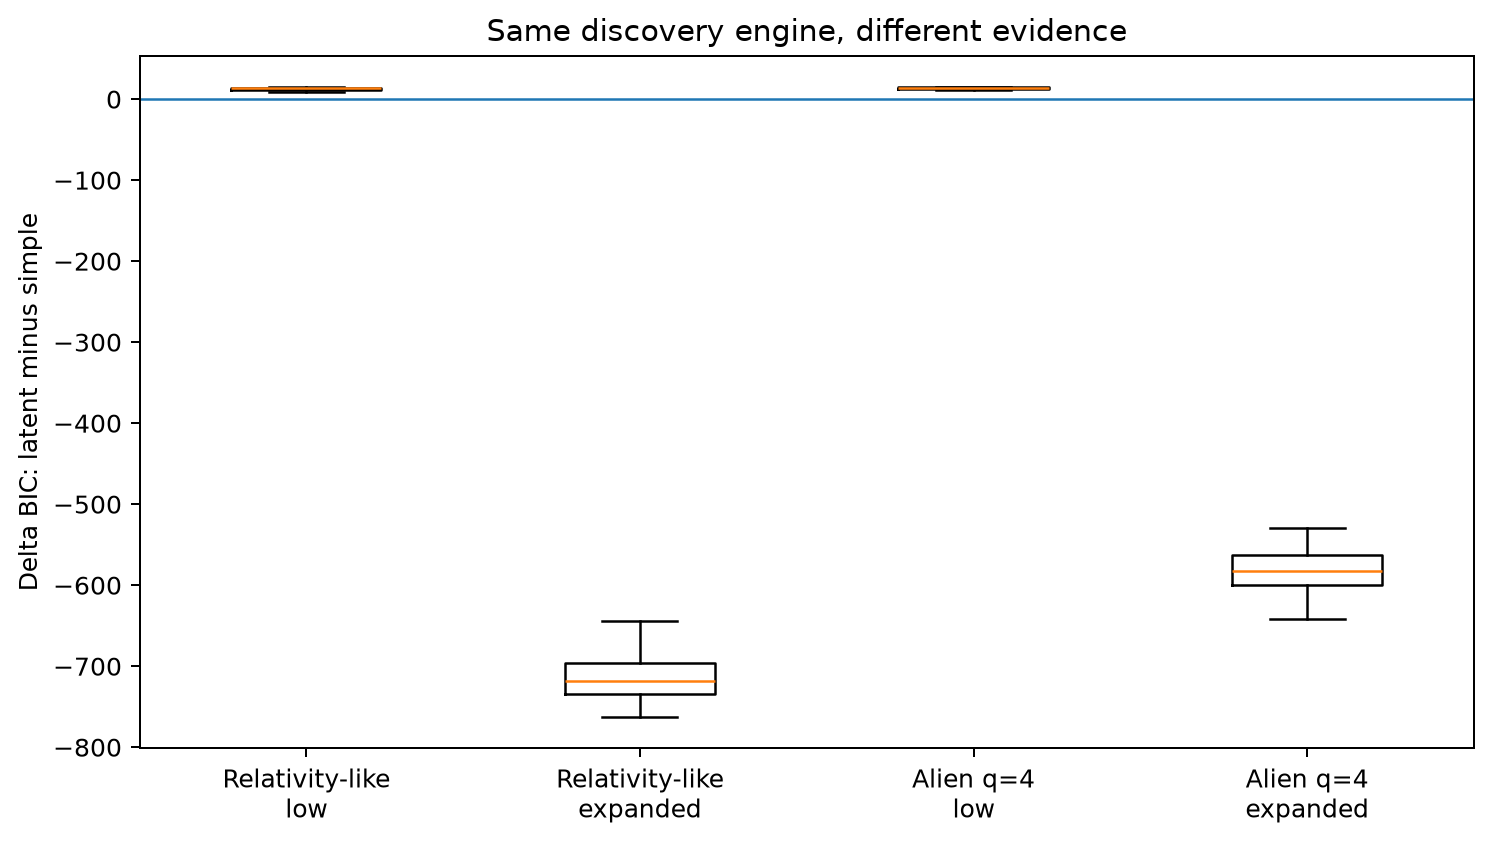
\includegraphics[width=0.88\textwidth]{figures/figure_evidence_ceiling.png}
\caption{The same search procedure appears conceptually conservative or conceptually expansive depending only on whether the observations make the richer distinction consequential.}
\end{figure}

The lesson is simple: failure to infer richer structure from evidence that does not distinguish it is not evidence of incapacity. Sometimes the next scientific operation is not more reasoning. It is a better measurement.

\subsection*{Wall 2: the distinction exists, but search does not find it}
Across 84 hidden-rule worlds where the needed distinction could be constructed from the available grammar, consequence-targeted search reached 95.87\% mean held-out accuracy, compared with 85.57\% for the strongest raw-coordinate baseline. On fresh controls, the same candidate space collapsed toward chance when the selected distinction was made independent of the target consequence. The gain came from choosing distinctions that repaired consequential errors, not merely from generating many features.

\begin{figure}[ht]
\centering
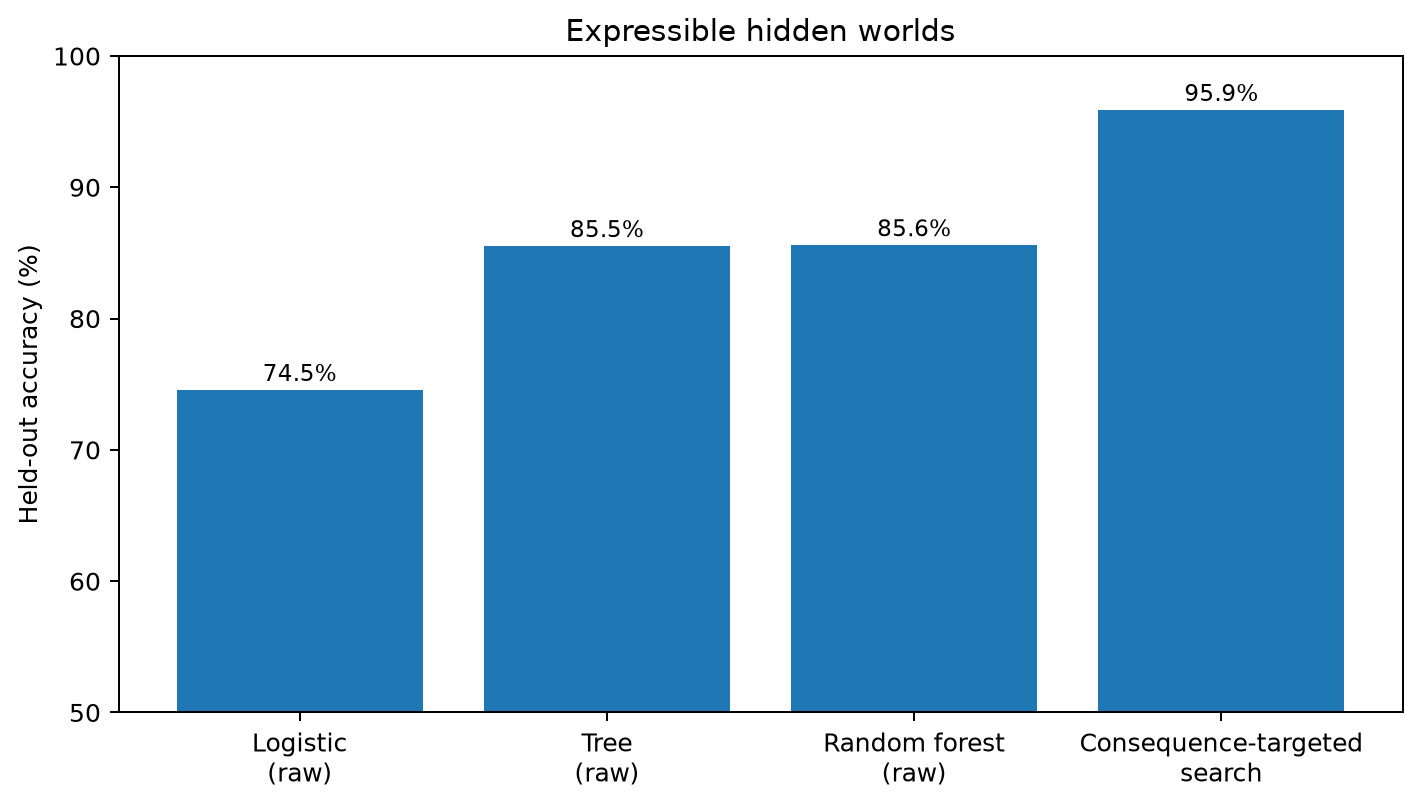
\includegraphics[width=0.80\textwidth]{figures/figure_ctds_expressible.png}
\caption{When the needed distinction is expressible, deliberately searching for consequence-changing distinctions can expose structure that ordinary prediction in the inherited coordinates underuses.}
\end{figure}

\subsection*{Wall 3: the language cannot state the distinction}
Then the experiment was made deliberately unfair in the opposite direction. The governing rules were chosen from primitive families absent from the candidate language. Mean balanced accuracy fell to 51.98\%, close to binary baseline. Searching harder inside the same language did not manufacture the missing primitive.

\begin{figure}[ht]
\centering
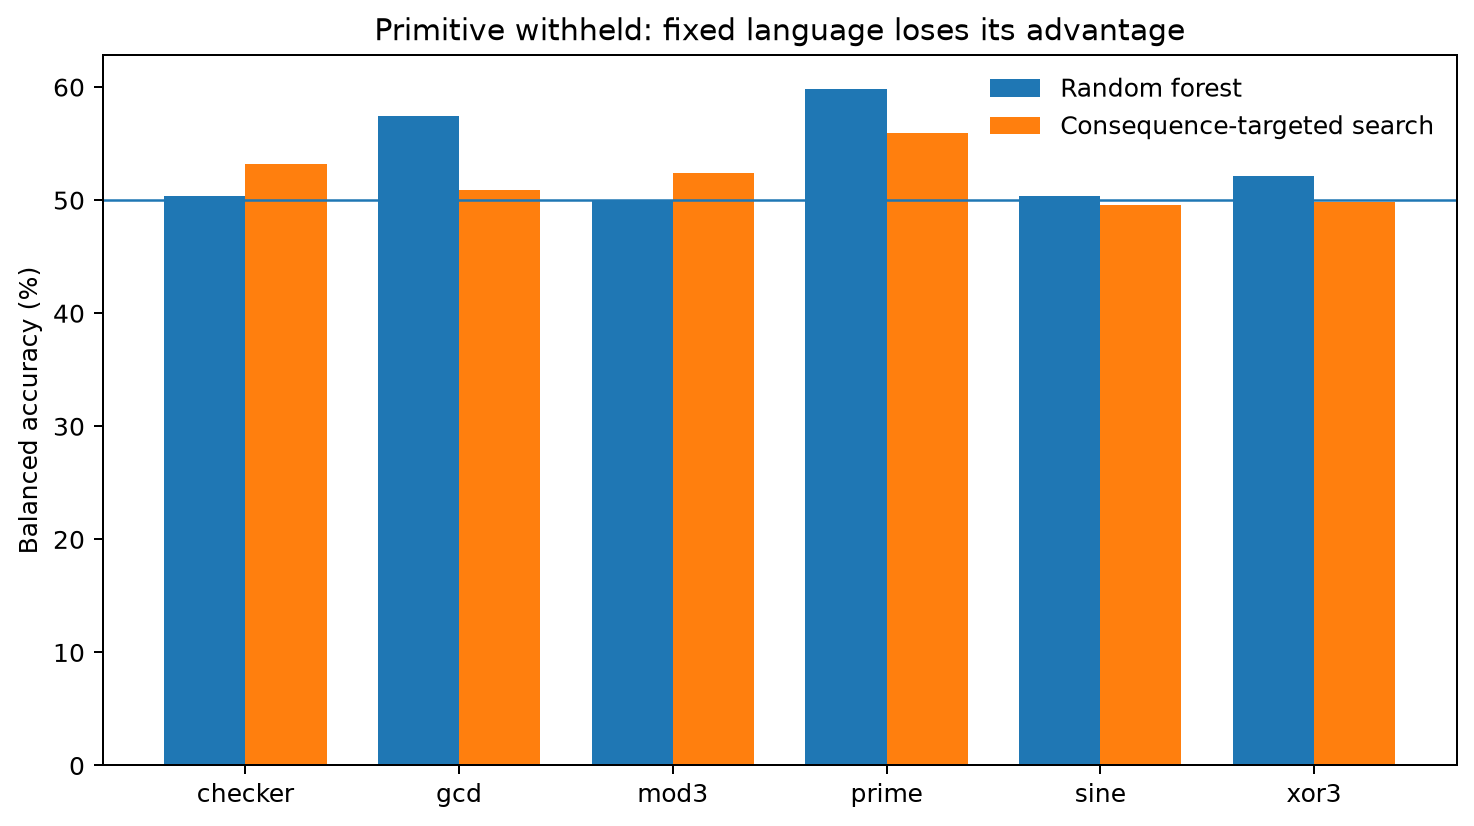
\includegraphics[width=0.82\textwidth]{figures/figure_primitive_ceiling.png}
\caption{When the governing primitive is withheld from the representation language, fixed-grammar search loses its advantage. A search failure and a language failure are not the same problem.}
\end{figure}

The combined result is more useful than a binary verdict about intelligence:

\begin{keybox}[Three ceilings]
\textbf{Evidence ceiling:} the world contains a distinction, but the observations do not make it consequential.\\
\textbf{Search ceiling:} the distinction is expressible, but the system does not find or select it.\\
\textbf{Language ceiling:} the distinction cannot be stated in the current representation language.
\end{keybox}

Each wall requires a different response. Change the measurement regime. Change the search. Or change the language in which search is allowed to occur.

\section{The Fourth Side: a representation escape you can see}
The dimensional claim becomes easier to understand when it is made executable.

Start with an impossible-looking projected figure. The construction used here solves three separate three-dimensional bars so that, from one selected viewing direction, their local occlusion relations form a cycle: $B$ lies over $A$, $C$ lies over $B$, and $A$ lies over $C$. No one of the six possible global depth orderings reproduces that projected reading. Yet the bars themselves are real, disjoint objects with a measured minimum gap of 0.283. From only 13 of 400 sampled directions does the object produce the impossible reading; from the other 387 it reads as ordinary separated bars.

This already exposes the central distinction. The contradiction belongs to a particular \emph{reading of a projection}, not to the existence of the object.

The construction is then embedded in four coordinates and the observer's displayed ``up'' direction is rotated through the plane spanned by the familiar vertical basis $e_2$ and a fourth spatial basis $u_w$:
\[
U(\alpha)=\cos\alpha\,e_2+\sin\alpha\,u_w.
\]
For an ordinary point whose fourth coordinate is zero, the displayed contribution becomes
\[
y\longmapsto y\cos\alpha.
\]
For displacement purely along the fourth coordinate,
\[
w\longmapsto w\sin\alpha.
\]

\begin{figure}[ht]
\centering
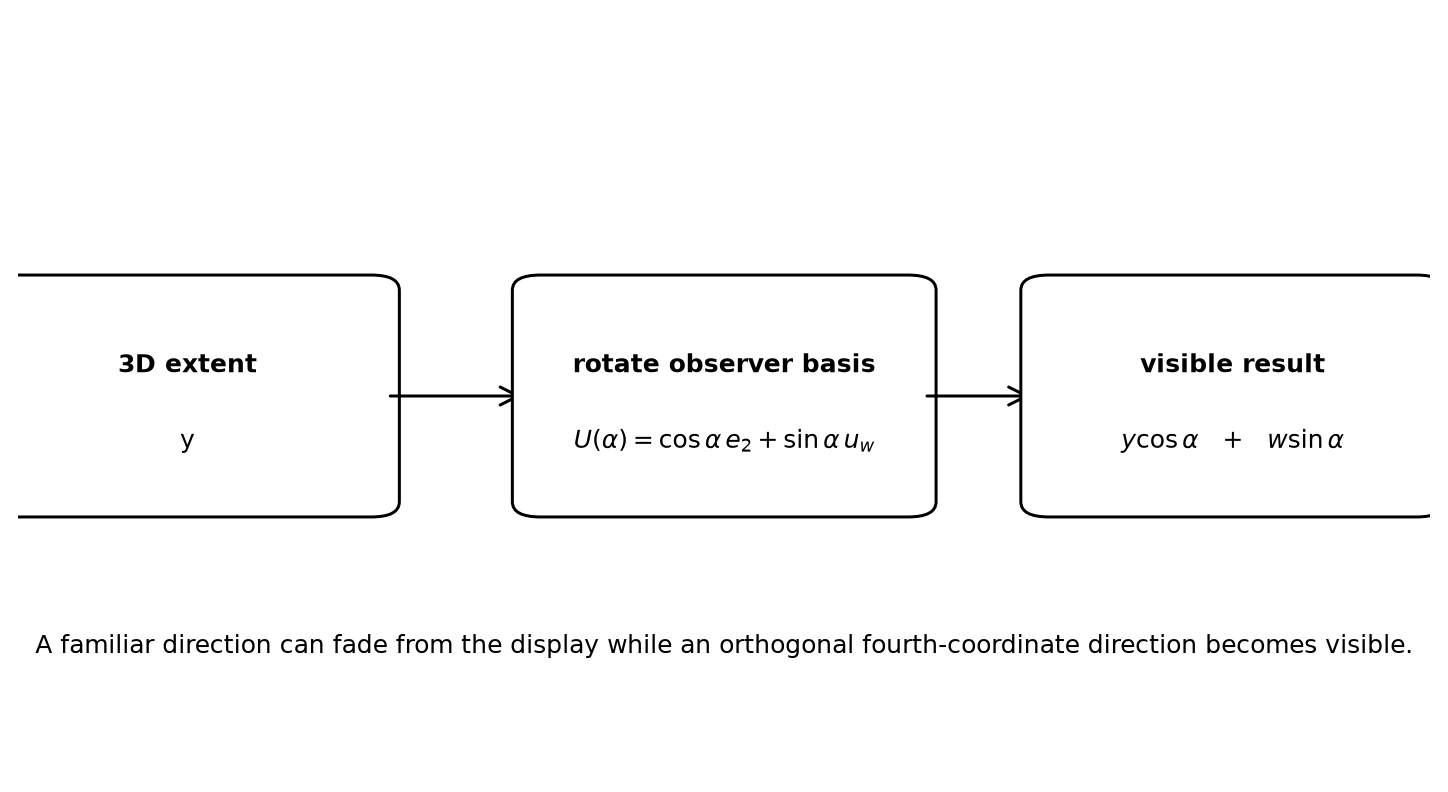
\includegraphics[width=0.92\textwidth]{figures/figure_fourth_side_schematic.png}
\caption{The apparently strange visual behavior is the expected behavior of the chosen four-dimensional basis rotation: familiar vertical extent is traded for visible fourth-coordinate extent.}
\end{figure}

At $\alpha=0$, the familiar vertical contribution is fully expressed and the longitudinal fourth-coordinate contribution is zero. Near $90^\circ$, the familiar contribution collapses while the fourth-coordinate contribution becomes fully expressed. Undoing the expected $\cos\alpha$ foreshortening reproduces the original three-bar projected figure at 100.000\% pixel identity for every tested angle in the canonical verification path.

Nothing in this result establishes that our physical universe contains an accessible fourth spatial dimension. That is not the claim. The claim is that a lower-dimensional physical system can construct, transform, and communicate a higher-dimensional representation, and that a human observer can acquire useful intuition about that representation through projection. The geometry of the display is not the geometry of the represented object, and the geometry of the represented object is not automatically the geometry of physical reality.

That distinction is precisely what representation escape needs.

\section{Representation is more than a list of variables}
The Fourth Side and AlexNet look unrelated only if a representation is defined as a coordinate vector. A broader object is needed.

Let
\[
\Rcal=(Z,\Gamma,\Pi),
\]
where $Z$ denotes the distinctions or latent variables carried by the representation, $\Gamma$ denotes which components may interact or communicate, and $\Pi$ denotes how internal state is exposed as predictions, measurements, or other relevant consequences.

\begin{figure}[ht]
\centering
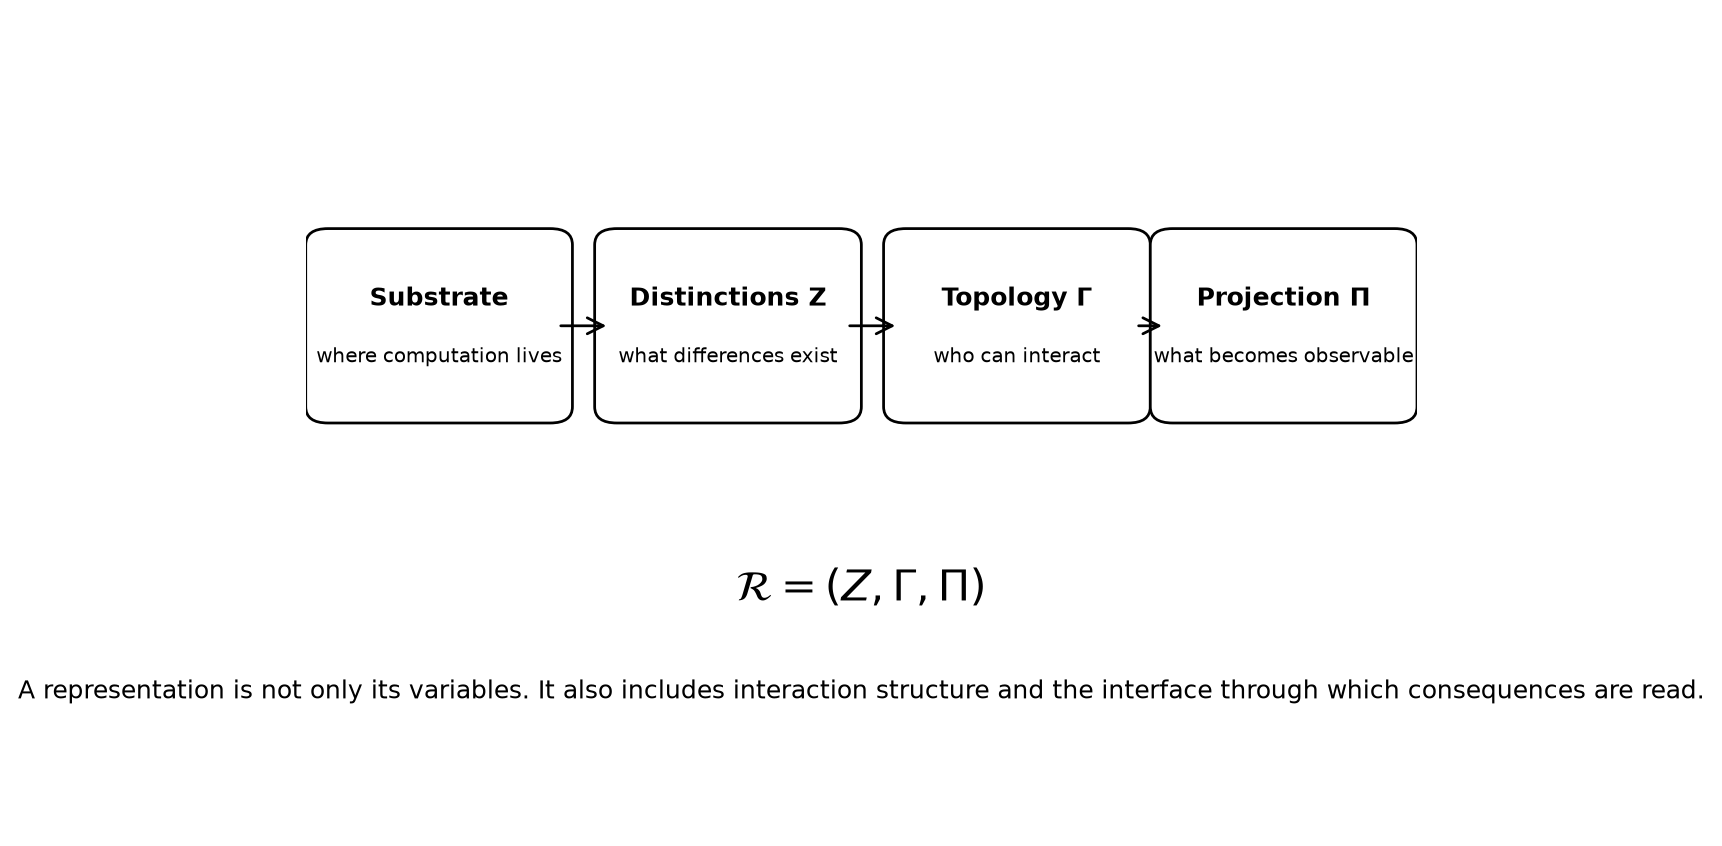
\includegraphics[width=0.88\textwidth]{figures/figure_representation_geometry.png}
\caption{Representation escape can alter what distinctions exist, which distinctions can interact, or how internal structure is projected into observable consequences.}
\end{figure}

This unifies several cases that otherwise look unrelated. Adding a fourth coordinate changes $Z$ and the observer interface $\Pi$. Splitting a model across devices changes $\Gamma$. A new instrument changes what part of the latent world is visible through $\Pi$. A new scientific concept changes $Z$. A new communication protocol changes $\Gamma$. A new measurement may make a previously useless distinction consequential without changing the world at all.

The consequence is a stronger definition of scientific progress. A representation should not be favored merely because it is familiar, historically successful, or easy for humans to picture. It should earn its structure through the consequences it preserves and the cost at which it preserves them.

\begin{keybox}[Representation escape]
A representation escape occurs when a system leaves an inherited representational commitment while preserving or improving the declared predictive and interventional consequences under an explicit cost and resource contract.
\end{keybox}

This makes ``impossible'' a dangerous word unless its frame is named. A more honest statement is often
\[
\operatorname{Impossible}(Y\mid \Rcal,B),
\]
meaning impossible under the current representation $\Rcal$ and resource envelope $B$. An absolute impossibility claim requires much more: a necessity argument showing that changing the representation cannot matter.

\section{The experiment we actually need}
The strongest test of machine scientific discovery is therefore not ``can the model rediscover Einstein?'' Rediscovery can still reward the historical human ontology.

A harder benchmark should hide the ontology itself. Remove canonical variable names, disciplinary labels, theory names, and privileged coordinate choices. Supply observations and interventions capable of separating rival worlds. Permit the system to add or delete coordinates, construct relational variables, alter communication structure, invent operators, and abandon geometric descriptions entirely when a non-geometric representation preserves the same consequences more cheaply.

Then change the constraints again.

Run the same underlying problem across different memory limits, communication graphs, observation interfaces, and substrate architectures. Ask what reappears. A decomposition that exists only because two GPUs could not share enough memory should disappear when that boundary disappears. A physical invariant should not care which GPU was available. A human-native coordinate system that repeatedly re-emerges across alien languages and substrates earns stronger evidence of structural privilege than one merely inherited from the benchmark designer.

This suggests a new empirical strategy: \emph{constraint sweeps}. Rather than testing one architecture under one resource envelope, vary the envelope deliberately and study the intersection of the structures that survive. The scientific target is not the first representation found. It is the structure that remains necessary across representational counterfactuals.

\begin{resultbox}[The inversion]
Representation escape is not an argument that human science is arbitrary. It supplies a stronger test for what is not arbitrary: change the path, the hardware, the language, the geometry, and the observation interface. Then ask what refuses to disappear.
\end{resultbox}

\section{Conclusion: science beyond the inherited interface}
Science has traditionally searched for better answers inside representations inherited from previous science, human language, biological perception, available instruments, and available machines. Those inheritances are often extraordinarily effective. Their success does not certify every part of them as necessary.

The argument of this paper can be stated compactly.

A successful historical path proves reachability, not necessity. A physical substrate does not bound the dimensionality of what it can computationally represent. A hardware partition may be a contingent response to memory rather than a property of the task. An observation may hide a distinction that a richer measurement would force. A search procedure may miss a distinction its language already permits. And a representation language may fail because the distinction reality requires is not expressible inside it at all.

These are not one mysterious ``jump.'' They are different ceilings with different remedies.

The deeper consequence is methodological. Scientific discovery should search not only over hypotheses, but over the representations in which hypotheses can exist. That means varying coordinates, primitives, interaction topology, projection, and resource constraints while holding the required consequences fixed. It means treating the geometry of the observer as one possible interface rather than an unquestioned boundary on thought. It means treating old impossibility claims as conditional whenever the capability or representation on which they depended has changed.

Most importantly, representation escape turns skepticism about inherited structure into a positive scientific test. If independent systems, using different substrates, languages, sensory projections, and search routes repeatedly converge on the same structure, then the case that the structure belongs to the world becomes stronger. If a distinction disappears as soon as an obsolete bottleneck is removed, then it belonged to the scaffolding.

Human science is one path through representation-space, walked by one kind of organism with one sensory history. The next frontier is not simply the set of questions that remain unanswered inside that path. It is the larger set of questions that become askable only after the representation itself changes.

\begin{keybox}[Research rule]
When progress stalls, do not ask only for more computation. Ask what is doing the limiting. If the evidence does not expose the distinction, change the measurement. If the distinction is available but buried, search for consequence-changing distinctions. If the language cannot state it, expand the language. If a boundary came from an old resource constraint, remove the constraint and test whether the boundary still earns its place. Then vary the representation again and look for what survives.
\end{keybox}

\appendix
\section{Methods and reproducibility in brief}
The main text deliberately emphasizes the scientific claims rather than implementation plumbing. The consequence-targeted search scripts, raw outputs, fixed seeds, and generated figures accompany the reproducibility package; the evidence-ceiling materials and The Fourth Side workspace remain referenced project artifacts.

\begin{itemize}[leftmargin=1.5em]
\item \textbf{Evidence ceiling.} A fixed model-selection engine compared a simple and richer law across 400 randomized trials while only the observational regime changed; all fitting rules and noise levels were held fixed.
\item \textbf{Expressible hidden-rule worlds.} Eighty-four randomized worlds contained hidden binary rules constructible from a bounded candidate grammar; one consequence-targeted derived distinction was selected on training data and evaluated once on a wider held-out distribution.
\item \textbf{Controls.} On 84 fresh worlds the same candidate space was retained while final selection was made target-independent or against shuffled labels, separating useful search from mere candidate proliferation.
\item \textbf{Primitive-withheld worlds.} Thirty-six worlds required rule primitives deliberately omitted from the candidate language; balanced accuracy was used because several families were class-imbalanced.
\item \textbf{The Fourth Side.} The canonical solver constructs three disjoint bars, verifies the cyclic projected reading and viewpoint census, then evaluates the production $e_2$--$w$ observer-basis rotation; legacy workspace paths that disagree with the canonical solver are not used as evidence.
\end{itemize}

The reproducibility artifacts should be read as tests of the claims above, not as a claim that the bounded algorithms constitute open-ended autonomous science. The experiments isolate mechanisms; the larger representation-escape benchmark remains a research target.

\section*{References}
\small
\begin{enumerate}[label={[\arabic*]},leftmargin=2.2em]
\item Fang, Y.-L., Jian, D.-S., Li, X., \& Ma, Y.-Q. (2025). AI-Newton: A Concept-Driven Physical Law Discovery System without Prior Physical Knowledge. arXiv:2504.01538.
\item Schmidt, M., \& Lipson, H. (2009). Distilling Free-Form Natural Laws from Experimental Data. \emph{Science} 324, 81--85.
\item Bongard, J., \& Lipson, H. (2007). Automated reverse engineering of nonlinear dynamical systems. \emph{PNAS} 104, 9943--9948.
\item Iten, R. et al. (2020). Discovering Physical Concepts with Neural Networks. \emph{Physical Review Letters} 124, 010508.
\item Littman, M. L., Sutton, R. S., \& Singh, S. (2001). Predictive Representations of State. NeurIPS 14.
\item Shalizi, C. R., \& Crutchfield, J. P. (2001). Computational Mechanics: Pattern and Prediction, Structure and Simplicity. \emph{Journal of Statistical Physics} 104, 817--879.
\item Ferns, N., Panangaden, P., \& Precup, D. (2011). Bisimulation Metrics for Continuous Markov Decision Processes. \emph{SIAM Journal on Computing} 40(6), 1662--1714.
\item Tishby, N., Pereira, F. C., \& Bialek, W. (1999/2000). The Information Bottleneck Method. 37th Allerton Conference; arXiv:physics/0004057.
\item Zahavy, T. (2026). Position: LLMs Can't Jump. ICML 2026 Position Track; OpenReview klU4737opt.
\item Penad\'es, J. R. et al. (2025). AI mirrors experimental science to uncover a mechanism of gene transfer crucial to bacterial evolution. \emph{Cell} 188(23), 6654--6665.e2.
\item Cook, M. (2004). Universality in Elementary Cellular Automata. \emph{Complex Systems} 15(1), 1--40.
\item Krizhevsky, A., Sutskever, I., \& Hinton, G. E. (2012). ImageNet Classification with Deep Convolutional Neural Networks. \emph{Advances in Neural Information Processing Systems} 25.
\end{enumerate}

\end{document}